\documentclass{standalone}
\usepackage{tikz}
\usepackage{ctex,siunitx}
\setCJKmainfont{Noto Serif CJK SC}
\usepackage{tkz-euclide}
\usepackage{amsmath}
\usetikzlibrary{patterns, calc,3d}
\usetikzlibrary {decorations.pathmorphing,decorations.pathreplacing,decorations.shapes}
\begin{document}
\small
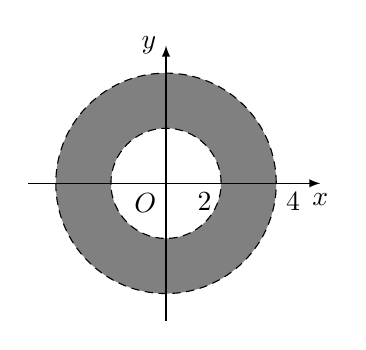
\begin{tikzpicture}[>=latex,scale=0.7]
  \draw[densely dashed,even odd rule,fill=gray](0,0)circle(2)(0,0)circle(1);
  \draw[->](-2.5,0)--(2.8,0)node[below]{$x$};
  \draw[->](0,-2.5)--(0,2.5)node[left]{$y$};
  \node at (0,0)[below left]{$O$};
  \node at (2,0)[below right]{4};
  \node at (1,0)[below left]{2};
\end{tikzpicture}
\end{document}